\documentclass[zihao=false,fontset=windows]{ctexart}
% ctexart 不接受任意 pt 选项。正文改 {10pt}，方括号里是行距。
\usepackage{scrextend}
\changefontsizes[12pt]{10pt}

\usepackage[a4paper,left=2.35cm,right=2.35cm,top=1.7cm,bottom=1.9cm]{geometry}
\usepackage{xcolor}
\usepackage{graphicx}
\usepackage{amsmath,amssymb}
\usepackage{enumitem}
\usepackage{tabularx}
\usepackage{colortbl}
\usepackage{listings}
\usepackage{hyperref}
\usepackage[most]{tcolorbox}

\definecolor{feishuText}{RGB}{31,35,41}
\definecolor{feishuBlue}{RGB}{36,91,219}
\definecolor{feishuRed}{RGB}{216,57,49}
\definecolor{feishuGreen}{RGB}{46,161,33}
\definecolor{feishuGray}{RGB}{100,106,115}
\definecolor{feishuGray2}{RGB}{143,149,158}
\definecolor{feishuPinkBg}{RGB}{251,191,188}
\definecolor{quoteBar}{RGB}{51,112,255}
\definecolor{codebg}{RGB}{245,246,247}
\definecolor{codeborder}{RGB}{222,224,227}
\definecolor{inlinebg}{RGB}{242,243,245}
\definecolor{callRed}{RGB}{253,226,226}
\definecolor{callOrange}{RGB}{255,245,235}
\definecolor{callYellow}{RGB}{254,255,240}
\definecolor{callGreen}{RGB}{240,251,239}
\definecolor{callBlue}{RGB}{240,244,255}
\definecolor{callRedSoft}{RGB}{254,241,241}
\definecolor{callSun}{RGB}{255,255,204}
\definecolor{callGreenPage}{RGB}{217,245,214}
\definecolor{callOrangePage}{RGB}{254,234,210}
\definecolor{callLilac}{RGB}{246,241,254}
\definecolor{tableHead}{RGB}{242,243,245}
\definecolor{tableRule}{RGB}{222,224,227}
\definecolor{codeText}{RGB}{31,35,41}
\definecolor{codeKeyword}{RGB}{0,0,255}
\definecolor{codeComment}{RGB}{0,128,0}
\definecolor{codeString}{RGB}{163,21,21}

\setmainfont{Times New Roman}
\setCJKmainfont{Microsoft YaHei}[AutoFakeBold=2.2]
\setCJKsansfont{Microsoft YaHei}[AutoFakeBold=2.2]
\setCJKmonofont{Microsoft YaHei}[AutoFakeBold=2.2]
\setmonofont{Consolas}
\newfontfamily\emojifont{Segoe UI Emoji}
\newfontfamily\symbolfont{Segoe UI Symbol}

\hypersetup{
  colorlinks=true,
  urlcolor=feishuBlue,
  linkcolor=feishuBlue,
  unicode=true,
  pdftitle={CoCa(2022, Google Research)}
}

\setlength{\parindent}{0pt}
\setlength{\parskip}{0.42em}
\setlength{\fboxsep}{1.5pt}
\setlength{\emergencystretch}{3em}
\linespread{1.28}
\color{feishuText}
\arrayrulecolor{tableRule}
\urlstyle{same}

\setlist[enumerate]{label=\textcolor{feishuBlue}{\arabic*.}, leftmargin=1.7em, itemsep=0.22em, topsep=0.28em, parsep=0.08em, partopsep=0pt}
\setlist[itemize,1]{label=\textcolor{feishuBlue}{\textbullet}, leftmargin=1.35em, itemsep=0.18em, topsep=0.25em, parsep=0.06em, partopsep=0pt}
\setlist[itemize,2]{label=\textcolor{feishuBlue}{◦}, leftmargin=1.45em, itemsep=0.12em, topsep=0.15em}
\setlist[itemize,3]{label=\textcolor{feishuBlue}{\rule[0.18em]{0.38em}{0.38em}}, leftmargin=1.55em, itemsep=0.1em, topsep=0.12em}

\newcommand{\feiEmoji}[1]{{\emojifont #1}}
\newcommand{\incode}[1]{\colorbox{inlinebg}{\ttfamily\small #1}}
\newcommand{\bigmath}[1]{%
  \begin{center}\large$\displaystyle #1$\end{center}%
}
\newcommand{\feiCirc}{\textcolor{feishuBlue}{◦}}
\newcommand{\feiSq}{\textcolor{feishuBlue}{\rule[0.18em]{0.38em}{0.38em}}}
\newcommand{\feiDot}{\textcolor{feishuBlue}{\textbullet}}

\lstset{
  language=Python,
  basicstyle=\ttfamily\footnotesize\color{codeText},
  keywordstyle=\color{codeKeyword},
  commentstyle=\color{codeComment},
  stringstyle=\color{codeString},
  showstringspaces=false,
  breaklines=true,
  columns=fullflexible,
  keepspaces=true,
  tabsize=4,
  upquote=true,
  aboveskip=2pt,
  belowskip=0pt,
  xleftmargin=0pt,
  frame=none
}

\tcbset{
  feishubase/.style 2 args={
    enhanced,
    boxrule=0pt,
    arc=8pt,
    left=10pt,
    right=10pt,
    top=7pt,
    bottom=7pt,
    before skip=6pt,
    after skip=6pt,
    colback=#1,
    colframe=#1,
    before upper={\feiEmoji{#2}\hspace{0.45em}\ignorespaces}
  }
}
\newtcolorbox{feishubox}[2]{feishubase={#1}{#2}, breakable}
\newtcolorbox{feishuboxnb}[2]{feishubase={#1}{#2}}

\newtcolorbox{feishuquote}{
  enhanced,
  breakable,
  boxrule=0pt,
  leftrule=3pt,
  arc=0pt,
  colframe=quoteBar,
  colback=white,
  left=8pt,
  right=2pt,
  top=2pt,
  bottom=2pt,
  before skip=4pt,
  after skip=4pt,
  before upper=\color{feishuGray}
}
\newtcolorbox{feishuquotenb}{
  enhanced,
  boxrule=0pt,
  leftrule=3pt,
  arc=0pt,
  colframe=quoteBar,
  colback=white,
  left=8pt,
  right=2pt,
  top=2pt,
  bottom=2pt,
  before skip=4pt,
  after skip=4pt,
  before upper=\color{feishuGray}
}

\newtcolorbox{feishuhigh}[1]{
  enhanced,
  breakable,
  boxrule=0pt,
  arc=8pt,
  colback=#1,
  colframe=#1,
  left=10pt,
  right=10pt,
  top=5pt,
  bottom=5pt,
  before skip=3pt,
  after skip=3pt
}

\newtcolorbox{feishucode}{
  enhanced,
  breakable,
  colback=codebg,
  colframe=codeborder,
  boxrule=0.6pt,
  arc=6pt,
  left=6pt,
  right=6pt,
  top=5pt,
  bottom=4pt,
  before skip=6pt,
  after skip=6pt
}

\newcommand{\codehead}{{\small\ttfamily\color{feishuGray}代码块}\par\vspace{-0.15em}}
\newcommand{\chip}[2]{%
  \begin{center}
  \tcbox[
    on line,
    colback=#1,
    colframe=#1,
    boxrule=0pt,
    arc=7pt,
    left=6pt,
    right=6pt,
    top=3pt,
    bottom=3pt,
    halign=center,
    before skip=0pt,
    after skip=0pt
  ]{\parbox{0.94\linewidth}{\centering\bfseries #2}}
  \end{center}%
}

\begin{document}
{\zihao{1}\bfseries CoCa(2022, Google Research)\par}

\begin{feishuquote}
CoCa：加快模型训练(2022, Google Research)\par
\textbf{Contrastive Captioners} are Image-Text Foundation Models\par
\end{feishuquote}

\begin{center}
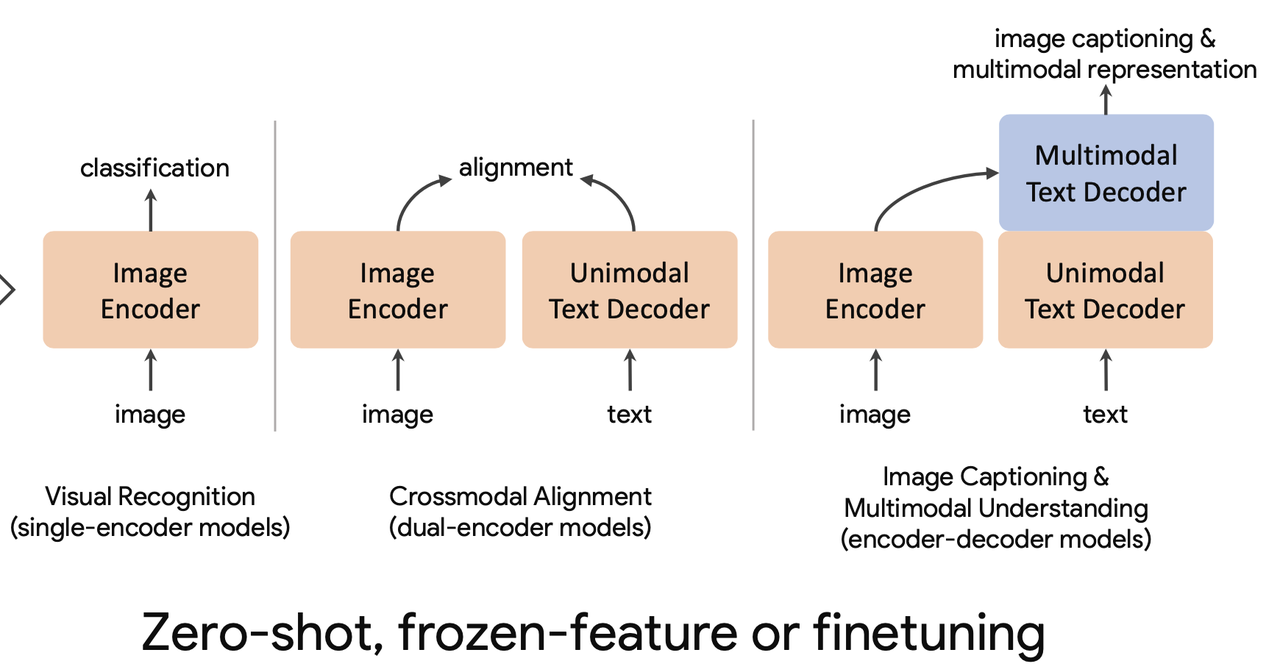
\includegraphics[width=0.98\textwidth]{images/2022-CoCa/fig-01.png}
\end{center}

用自然语言作为监督信号的三种基本方法：\par

{\renewcommand{\tabularxcolumn}[1]{>{\raggedright\arraybackslash}m{#1}}%
\renewcommand{\arraystretch}{1.25}%
\setlength{\tabcolsep}{3.5pt}%
\begin{tabularx}{\textwidth}{|X|X|X|}
\hline
\chip{callGreen}{Single(Fusion)-encoder model}
&
\chip{callBlue}{Dual-encoder model}
&
\chip{callLilac}{Encoder-decoder model}
\\
\hline
在\textbf{手工标注的干净的数据集}上通过图像分类任务预训练一个\textbf{视觉编码器}，训练损失为交叉熵损失。\par
只能去做一些视觉方面的任务，并不能做多模态任务。
&
不再需要手工标注的干净的数据集，而是\textbf{借助大量带噪声的网络上的图像文本对}，通过对比损失预训练 \textbf{Dual-Encoder 的视觉模型和语言模型}。\par
在一些下游任务中，比如zero-shot图像分类或者图文检索任务，可以获得很好的效果。但是这种方法图像和文本独立编码，且编码过程中并没有任何图像和文本侧的交叉，只在最后计算cosine相似度，缺少图像和文本的融合表示，因此不适用于VQA等需要对图像和文本联合理解的任务
&
\textbf{生成式任务}，也叫描述任务，要求\textbf{模型以自回归的方式根据上文来推测下文是什么}。模型的架构是 \textbf{Encoder-Decoder 类型}，这种类型的模型架构可以\textbf{联合学习视觉和多模态的特征}。在预训练期间，模型在 Encoder 端 (可以使用 Vision Transformer 或 ConvNet) 获取图像并编码图片的特征。Text Decoder 输出上使用语言建模 (LM) 损失函数，推测下文的输出。同时，解码器的输出也可以作为视觉语言的联合表征。
\\
\hline
\end{tabularx}}

\par\vspace{1.15em}\noindent{\zihao{-2}\bfseries 1. 概述}\par\vspace{0.28em}
CoCa 是一种多模态 Transformer 模型，顾名思义\textcolor{feishuRed}{\textbf{Contrastive Captioners}}，就是在训练的时候使用两个目标函数，分别是\textbf{基于对比学习的损失函数 Contrastive Loss（ITC）}和\textbf{基于生成式图像字幕任务的目标函数 Captioning Loss（LM）}。CoCa融合了上面3种模型结构，既能生成图像侧和文本侧独立的表示（CLIP），又能进行更深层次的图像、文本信息融合以及文本生成（Encoder-decoder），适用于更广泛的任务：包括 Image Encoder，单模态 Text Encoder 和多模态 MultiModal Encoder。\par
也可以简单认为CoCa是CLIP加上了一个image caption的预训练任务。Coca因此具备了三种能力，纯图像模型的表示生成，图文多模态表示对齐，图片描述生成(image caption)。\par
其实\textcolor{feishuBlue}{用单模态文本特征输入对齐图像特征的方式这种方法}在ALBEF中就使用过，类似也是先用对比损失对齐文本和图像特征，然后使用cross attention来辅助解码语言模型的预训练，不过CoCa并没有ALBEF的引用。其实CoCa可以算是ALBEF的一个后续工作。\par

\begin{feishubox}{callSun}{🌟}
\textcolor{feishuRed}{\textbf{主要贡献点：}}\par
\begin{enumerate}
\item 融合了三种基本模型结构的特点，\textbf{统一了对比学习和生成任务}，通过共享的编码器和解码器框架完成多任务学习，生成更为准确且多样的图像描述
\item 加快了训练速度，处理一个batch的图像-文本对\textbf{只需要前向和后向计算一次}（ALBEF需要两次）。
\end{enumerate}
\end{feishubox}

\par\vspace{1.15em}\noindent{\zihao{-2}\bfseries 2. 模型架构}\par\vspace{0.28em}
CoCa 以上面三种基础结构的优势为基础，使用带有解耦解码器的单个encoder-decoder Transformer来处理对比学习信号和生成学习信号。\par
CoCa的整体结构包括3个部分\textbf{：一个图像encoder（Image Encoder）和两个文本decoder（Unimodal Text Decoder、Multimodal Text Decoder）}。\textbf{Image Encoder端还有一个Attentional Pooling。}\par
\begin{feishuquote}
整个结构看作是一个encoder-decoder Transformer，encoder端是视觉的，decoder端是文本的，然后有将decoder切分成2部分，后面的部分有cross attention，前面部分没有。\par
\end{feishuquote}

\begin{center}
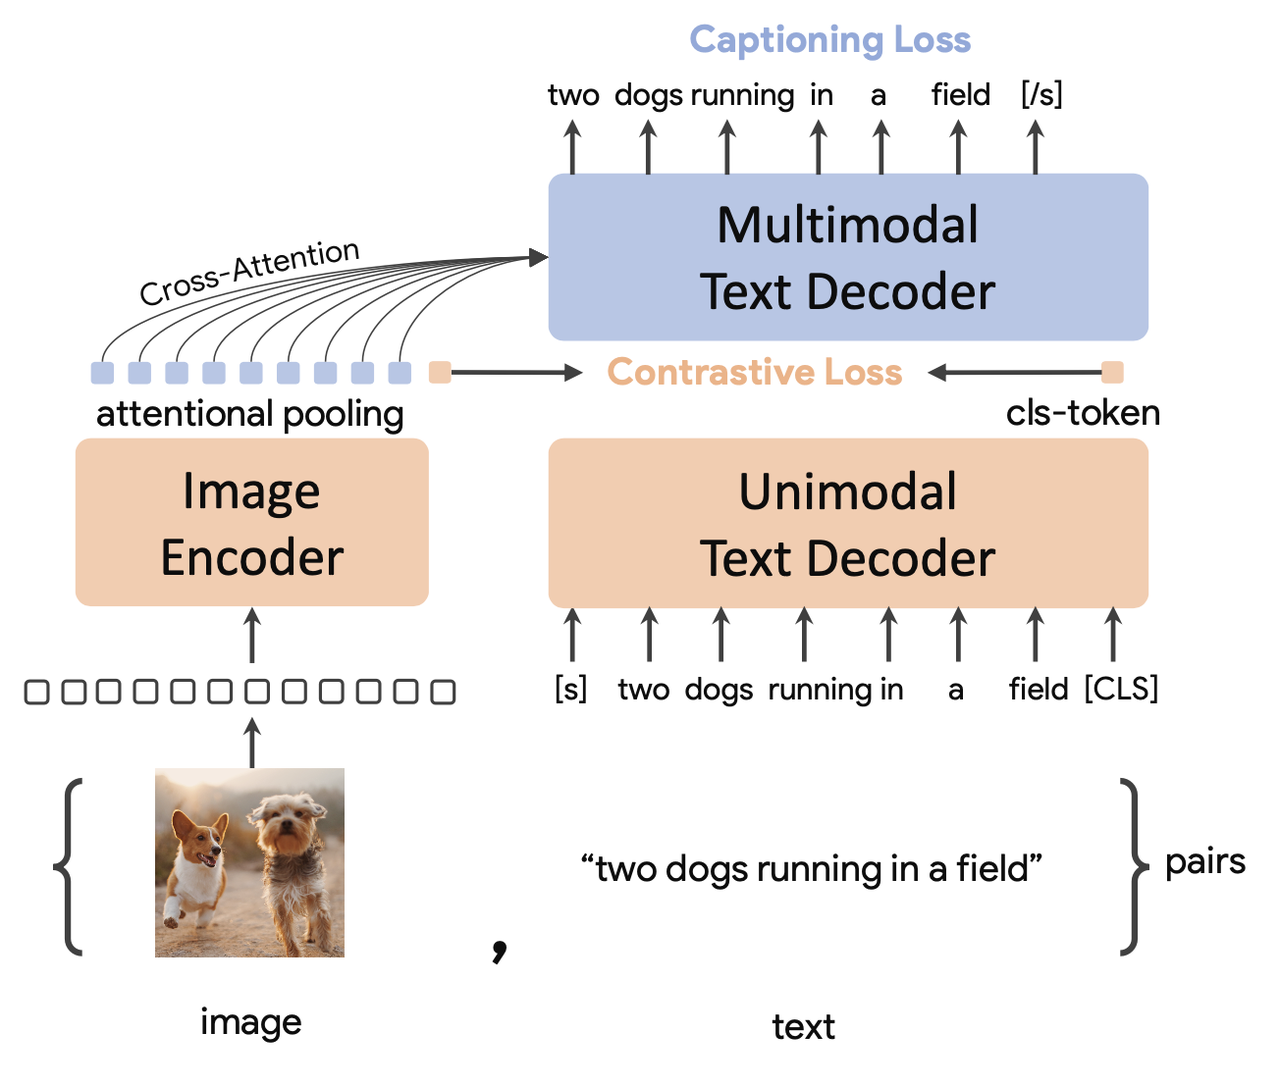
\includegraphics[width=0.98\textwidth]{images/2022-CoCa/fig-02.png}
\end{center}

\begin{enumerate}
\item Image Encoder 图像编码器\par
类似于Single-encoder 模型的工作方式
\begin{itemize}[label=\feiCirc, leftmargin=1.45em]
\item 使用一个视觉变换器（\feiEmoji{🌰} ViT，默认为ViT，也可以使用其他CNN）对输入图像进行编码，生成一系列图像特征表示img\_embed
\item img\_embed通过\textcolor{feishuRed}{\textbf{注意力池化attentional pooling}}进一步提取，分别生成两个特征：
\begin{itemize}[label=\feiSq, leftmargin=1.55em]
\item \textbf{对比特征 (Contrastive Feature, con\_feature)}： 专门的 \textbf{[cls]token} ，用于对比学习，通过与文本的[cls]特征进行对比。
\item \textbf{描述特征 (Captioning Feature, cap\_feature)}： 除了[cls]，其他的图像特征经过 attentional pooling 后，传入多模态 Text Decoder中，用于文本生成任务，作为多模态解码器的输入。
\end{itemize}
\begin{feishuquotenb}
\textcolor{feishuRed}{\textbf{attentional pooling}}\par
（源自于Set Transformer，其实作用类似于BLIP-2中的Q-Former，作为bottleneck，将信息进行进一步的提取，把最有用的信息融合在更少的token中）\par
\textbf{设计原因}：image-encoder侧的信息既可以提取一个统一的[cls]表示，也可以提取每个token的表示，二者各有不同的适用场景（\textcolor{feishuBlue}{单个[cls]token可作为视觉识别任务的全局表示，而使用更多视觉tokens可提供更精细的细节，这对于需要区域级特征的多模态任务很有帮助}），所以CoCa 采用特定于任务的attentional pooling来为不同的训练目标和下游任务定制\textbf{视觉表示}。\par
\textbf{原理}：可学习的，由\textbf{multi-head attention}实现，用于对image-encoder的输出进行处理，根据特定任务进行特征聚合。其中，query是预先定义的一个可训练的embedding（根据不同任务，这个query不同），key和value是image encoder的输出（img\_embed）。\par
\begin{itemize}[label=\feiDot, leftmargin=1.35em]
\item 对于\textcolor{feishuRed}{\textbf{对比学习}}任务，采用\textbf{维度为1的query}进行attention，将img\_embed融合为\textbf{单个向量表示[cls]}，表示\textbf{图像全局信息}，以支持与文本端文本全局特征的对比学习任务。\par
con\_feature = attentional\_pooling(img\_feature, con\_query)
\item 对于\textcolor{feishuRed}{\textbf{生成任务}}，采用\textbf{维度为256的query}进行attention，将img\_embed生成\textbf{更多的视觉tokens表示更多精细的细节}，以此和文本特征进行多模态融合。\par
cap\_feature = attentional\_pooling(img\_feature, cap\_query)
\end{itemize}
\end{feishuquotenb}
\end{itemize}

\item Unimodal Text Decoder 单模态文本解码器
\begin{itemize}[label=\feiCirc, leftmargin=1.45em]
\item 处理纯文本信息（不参与对图像特征的cross-attention，不受图像影响）
\item 文本输入时添加一个[cls]token，输入到tranformer中进行编码，输出一个text\_embed，其中最后一个[cls]代表文本的全局信息。
\item 这个文本[cls]与上面的图片[cls]用于ITC loss，然后text\_embed其余部分输入到Multimodal Text Decoder用于融合多模态信息。
\item \feiEmoji{⚠} 单向decoder，用的是casual attention（Masked），为防止信息泄漏，只能看到序列前面的部分
\end{itemize}

\item Multimodal Text Decoder 多模态文本解码器
\begin{itemize}[label=\feiCirc, leftmargin=1.45em]
\item 输入：\textbf{图像的描述特征（cap\_feature） + 上一步text\_embed（除去[cls]）}
\item 利用\textbf{cross attention}，\textbf{生成与图像内容相关的描述（Caption）（/还原对应文本）}，实现对视觉和语言的联合理解。
\item 输出文本序列，优化目标为\textbf{描述生成损失 (Captioning Loss)——LM loss}。
\item \feiEmoji{⚠} 单向decoder，用的是casual attention（Masked），为防止信息泄漏，只能看到序列前面的部分
\end{itemize}
\end{enumerate}

\begin{feishubox}{callOrangePage}{⚠}
\begin{enumerate}
\item 文本端，Unimodal Text Decoder和Multimodal Text Decoder的\textbf{层数是相同的}，也就是把一个transformer解码器平均分为两部分，因为浅层的早期融合对于多模态理解也可能是不必要的。
\item CoCa中Decoder部分所有的\textbf{自注意力都是用了掩码操作}的，对于一个批量的图像文本对，只进行\textcolor{feishuRed}{\textbf{一次}}前向传播和反向传播，和一些需要多阶段训练的模型相比，这就带来了效率上的提升。
\end{enumerate}
\end{feishubox}

CoCa和ALBEF其实是很像的，他们都采用 “图像分支 + 文本分支” 的结构，左边是\textbf{图像编码器} (Image Encoder)，右边是\textbf{文本处理器} (Text Branch)。都是在文本分支中的后一部分使用cross attention将图像信息和文本信息进行融合。\par
但也是文本分支中，ALBEF使用Encoder来处理，CoCa则使用Decoder来处理。\par
\begin{feishuquote}
Decoder 的意义：CoCa 的 Decoder 更倾向于语言生成任务（LM），不仅能抽取文本特征，还能自然支持语言生成任务（如 Captioning）。\par
Encoder 的意义：ALBEF 的 Encoder 主要用于文本特征的理解，适用于ITC任务。\par
\end{feishuquote}
所以ALBEF 在每个 iteration 训练的时候，文本部分的模型要 forward 2次，一次是输入完整的文本做图文匹配任务，一次是输入 mask 之后的文本做完形填空任务。\par
但是CoCa只需要1次前向和反向，即可同时计算ITM loss和LM loss。\par

\begin{feishubox}{callGreenPage}{🙋}
解耦解码器的作用：\par
\begin{feishuquotenb}
CoCa中\textbf{解耦的解码器结构（decoupled decoder architecture）：}\par
解耦：在模型内部对不同任务的功能与特征进行明确分离的设计方式\par
\begin{enumerate}
\item \textbf{输入信息的解耦}：\par
单模态解码器与多模态解码器分别处理不同类型的信息，前者纯粹用于文本特征提取（对比任务），后者用于视觉-文本的联合理解与生成任务。
\item \textbf{训练目标的解耦}：\par
单模态解码器产生的文本特征用于对比学习任务，而多模态解码器则专注于生成任务（如图像描述）。两个解码器可以独立地计算不同的损失函数，这样两类任务的训练就能高效且互不干扰地进行。
\end{enumerate}
\end{feishuquotenb}
\textbf{高效性}：模型只需一次前向传播就能同时完成对比任务和生成任务，而无需分别进行多次独立计算。\par
\textbf{灵活性}：两个子解码器能分别针对各自任务优化，不会因信息互相干扰而降低性能。\par
\textbf{泛化性}：单模态文本解码器学到纯粹的文本表示，而多模态解码器则能够有效地融合图像和文本的表示，从而提升CoCa在不同任务场景下的泛化能力。\par
\end{feishubox}

\par\vspace{1.15em}\noindent{\zihao{-2}\bfseries 3. 预训练}\par\vspace{0.28em}
在训练过程中，CoCa采用了两个个核心的训练目标：ITC、LM\par
\textcolor{feishuRed}{\textbf{CoCa综合训练目标}}：$L_{CoCa}=\lambda_{Con}L_{Con}+\lambda_{Cap}L_{Cap}$，其中：$\lambda_{Con}$ 与 $\lambda_{Cap}$ 是用于调节ITC loss和LM loss之间权重的超参数。\par

\begin{itemize}
\item \textbf{双编码器对比学习目标（Dual-Encoder Contrastive Learning）：}\textcolor{feishuRed}{\textbf{ITC loss}}\par
\textcolor{feishuGreen}{用于优化\textbf{图像编码器}和\textbf{单模态文本解码器}在多模态嵌入空间中的对齐。}
\begin{itemize}
\item \textcolor{feishuRed}{\textbf{从头开始训练}}
\item who参与ITC对比学习：
\begin{itemize}
\item image-encoder的输出经过一个Attentional Poolling后输出的\textcolor{feishuBlue}{\textbf{单个图像[cls] token}}
\item Unimodal Text Decoder的输出中最后的单个\textcolor{feishuBlue}{\textbf{文本[cls] token}}
\end{itemize}
\end{itemize}

\item \textbf{编码器-解码器描述生成目标（Encoder-Decoder Captioning）：}\textcolor{feishuRed}{\textbf{LM loss}}（BLIP、GPT系列用的Language Modeling Loss）\par
\textcolor{feishuGreen}{用于优化\textbf{图像编码器}和\textbf{多模态文本解码器}对生成任务（文本生成）的质量，使模型学习如何结合图像与文本特征，准确地进行图像描述生成和多模态任务的理解。}\par
LM loss：在已知图像特征和之前生成的所有词语的情况下，计算生成每个词语的负对数似然值（negative log-likelihood）。通过最小化该损失，CoCa能够逐步学会生成准确且连贯的图像描述。
\begin{itemize}
\item \textcolor{feishuRed}{\textbf{从头开始训练}}
\item who参与LM生成任务：
\begin{itemize}
\item image-encoder的输出经过一个Attentional Poolling后输出的\textcolor{feishuBlue}{\textbf{图像特征序列}}
\item Unimodal Text Decoder 输出的除去最后的[cls]token的\textcolor{feishuBlue}{\textbf{文本特征序列}}
\end{itemize}
\end{itemize}
\end{itemize}

\begin{feishuhigh}{callSun}
\textcolor{feishuRed}{\textbf{总结CoCa训练过程：}}
\end{feishuhigh}
\begin{feishuhigh}{callBlue}
\textcolor{feishuBlue}{1.} 图像通过Image Encoder（ViT），得到一系列的图像特征token；
\end{feishuhigh}
\begin{feishuhigh}{callBlue}
\textcolor{feishuBlue}{2.} 对图像特征进行attention pooling（multihead attention）, 取第0位作为计算对比损失的[cls]token，后255位作为计算生成损失的视觉token；
\end{feishuhigh}
\begin{feishuhigh}{callBlue}
\textcolor{feishuBlue}{3.} 文本（在最后添加[cls]token）通过文本的解码器，得到一系列的文本特征token。
\end{feishuhigh}
\begin{feishuhigh}{callBlue}
\textcolor{feishuBlue}{4.} 图像的[cls]token和文本的[cls]token计算ITC loss
\end{feishuhigh}
\begin{feishuhigh}{callBlue}
\textcolor{feishuBlue}{5.} 图像的视觉token和文本的其他token传到多模态的Text Decoder里做Cross Attention，融合视觉和文本的特征。多模态的特征用Captioning Loss（LM）训练。
\end{feishuhigh}

伪代码：\par
\begin{feishucode}
\codehead
\begin{lstlisting}
# 输入数据说明：
# image: 输入图像数据
# text.ids: 输入文本对应的token id序列
# text.labels: 文本的目标标签（用于caption生成的真实标签）
# text.mask: 文本掩码，表示有效token位置
# con_query: 对比学习的查询向量（用于生成对比特征）
# cap_query: 图像描述任务的查询向量（用于生成caption特征）
# cls_token_id: 词表中特殊的[CLS] token的id

# 注意力池化函数定义：
def attentional_pooling(features, query):
    # 使用多头注意力机制，以query为查询向量对特征进行池化
    out = multihead_attention(features, query)
    # 对注意力输出进行Layer Normalization，稳定训练过程
    return layer_norm(out)

# 将图像通过视觉Transformer（ViT）编码器，得到图像特征
img_feature = vit_encoder(image)  # 输出形状：[batch_size, 序列长度, 特征维度]

# 利用对比学习的单个查询向量（con_query）对图像特征进行池化，获得用于对比任务的图像表示
con_feature = attentional_pooling(img_feature, con_query)  # [batch_size, 1, 特征维度]

# 利用图像描述任务的多个查询向量（cap_query）对图像特征进行池化，获得用于caption任务的图像表示
cap_feature = attentional_pooling(img_feature, cap_query)  # [batch_size, N, 特征维度]

# 将文本的token序列和一个特殊的[CLS] token id拼接
ids = concat(text.ids, cls_token_id)

# 构造对应文本掩码，其中CLS token位置不需要额外mask（这里用0填充）
mask = concat(text.mask, zeros_like(cls_token_id))  # 去除CLS token的padding影响

# 将文本id序列转化为文本嵌入向量
txt_embs = embedding_lookup(ids)

# 单模态文本解码器（Unimodal Text Decoder）：仅对文本嵌入进行Transformer编码，不考虑图像特征
unimodal_out = lm_transformers(txt_embs, mask, cross_attn=None)

# 多模态文本解码器（Multimodal Text Decoder）：融合文本嵌入和图像特征（cap_feature）
# 输入时排除最后一个CLS token对应的输出
multimodal_out = lm_transformers(
    unimodal_out[:, :-1, :],  # 不包含最后一个CLS token的文本嵌入
    mask,
    cross_attn=cap_feature    # 与图像特征进行跨注意力融合
)

# 提取单模态文本解码器输出的最后一个token（即CLS token）特征，并进行Layer Normalization
cls_token_feature = layer_norm(unimodal_out)[:, -1:, :]  # [batch_size, 1, 特征维度]

# 计算对比学习损失（contrastive_loss），将图像特征(con_feature)和文本的CLS token特征进行对比
con_loss = contrastive_loss(con_feature, cls_token_feature)

# 计算图像描述（caption）任务的交叉熵损失（softmax cross entropy loss）
cap_loss = softmax_cross_entropy_loss(
    multimodal_out,
    labels=text.labels,  # caption任务对应的目标标签
    mask=text.mask       # mask用于指示有效的token位置
)

# 总体损失由以上两个损失组合而成
\end{lstlisting}
\end{feishucode}

\par\vspace{1.15em}\noindent{\zihao{-2}\bfseries 4. 模型实现代码}\par\vspace{0.28em}
Image Encoder\par
\begin{feishucode}
\codehead
\begin{lstlisting}
    def _encode_image(self, images, normalize: bool = True):
        image_latent, tokens_embs = self.visual(images)
        image_latent = F.normalize(image_latent, dim=-1) if normalize else image_latent
        # image_latent:constractive_token, tokens_embs: caption_token
        return image_latent, tokens_embs
        
    #### self.visual(images)：
    def forward(self, x: torch.Tensor):
        # [b, 3, 224, 224]--->[b, 1024, 16, 16]
        x = self.conv1(x)
        # [b, 1024, 16, 16]--->[b, 1024, 256]
        x = x.reshape(x.shape[0], x.shape[1], -1)
        # [b, 1024, 256]--->[b, 256, 1024]
        x = x.permute(0, 2, 1)

        # 在序列长度上给图像嵌入一个类别，x：[b, 256 + 1, 1024]
        x = torch.cat([_expand_token(self.class_embedding, x.shape[0]).to(x.dtype), x], dim=1)
        # 嵌入位置编码，x：[b, 256 + 1, 1024]
        x = x + self.positional_embedding.to(x.dtype)
        # patch_dropout， x：[b, 256 + 1, 1024]
        x = self.patch_dropout(x)
        # LayerNorm处理 x：[b, 256 + 1, 1024]
        x = self.ln_pre(x)
        # NLD -> LND [b, 256 + 1, 1024]---> [256 + 1, b, 1024]
        x = x.permute(1, 0, 2)
        # transformer网络处理
        x = self.transformer(x)
        # LND -> NLD  [256 + 1, b, 1024]--->[b, 256 + 1, 1024]
        x = x.permute(1, 0, 2)

        if self.attn_pool is not None:
                        # this is the original OpenCLIP CoCa setup, does not match paper
                        # x：[b, 257, 1024]--->[b, 256, 768]
                        x = self.attn_pool(x)
                        # ln归一化, [b, 256, 768]
                        x = self.ln_post(x)
                        # pooled: 类别token：[b, 768] tokens：图像token:[b, 255, 768]
                        pooled, tokens = self._global_pool(x)

        # pooled: [b, 768]@[768, 768]--->[b, 768]
        if self.proj is not None:
            pooled = pooled @ self.proj
        # 同时返回cls-token和视觉token
        if self.output_tokens:
                         return pooled, tokens
        
        return pooled
\end{lstlisting}
\end{feishucode}

Attentional Pooling\par
\begin{feishucode}
\codehead
\begin{lstlisting}
# self.attn_pool(x)
class AttentionalPooler(nn.Module):
    def __init__(
            self,
            d_model: int,
            context_dim: int,
            n_head: int = 8,
            n_queries: int = 256,
            norm_layer: Callable = LayerNorm
    ):
        super().__init__()
        self.query = nn.Parameter(torch.randn(n_queries, d_model))
        self.attn = nn.MultiheadAttention(d_model, n_head, kdim=context_dim, vdim=context_dim)
        self.ln_q = norm_layer(d_model)
        self.ln_k = norm_layer(context_dim)

    def forward(self, x: torch.Tensor):
        # ln归一化，NLD -> LND [b, 257, 1024]--->[257, b, 1024]
        x = self.ln_k(x).permute(1, 0, 2)
        N = x.shape[1]
        # q: [256, 768]
        q = self.ln_q(self.query)
        # q: [256, 768]--->[256, 1, 768]--->[256,b, 768], k=v=x, x:[257, b, 1024]
        # out: [256, b, 768]， MultiheadAttention
        out = self.attn(q.unsqueeze(1).expand(-1, N, -1), x, x, need_weights=False)[0]
        # out: [256, b, 768]--->[b, 256, 768]
        return out.permute(1, 0, 2)  # LND -> NLD
\end{lstlisting}
\end{feishucode}

Unimodal Text Decoder\par
\begin{feishucode}
\codehead
\begin{lstlisting}
    def _encode_text(self, text, normalize: bool = True):
        # text_latent:[b, 768], token_emb:[b, 76, 768]
        text_latent, token_emb = self.text(text)
        text_latent = F.normalize(text_latent, dim=-1) if normalize else text_latent
        return text_latent, token_emb

    def forward(self, text):
        cast_dtype = self.transformer.get_cast_dtype()
        seq_len = text.shape[1]
        # x：[b, 76, 768]， 将text：[b, 76]进行embeding， F.embedding(text, weight=[40408, 768]）49408---一共49408个单词，每个单词维度768
        x = self.token_embedding(text).to(cast_dtype)
        attn_mask = self.attn_mask
        if self.cls_emb is not None:
            seq_len += 1
            # 在文本token末尾嵌入cls_token, x:[b, 76, 768] ---> [b, 76+1, 768]
            x = torch.cat([x, _expand_token(self.cls_emb, x.shape[0])], dim=1)
            # cls_mask: [12b, 77, 77]， text：[b, 76]
            cls_mask = self.build_cls_mask(text, cast_dtype)
            # 将单词有序遮挡mask， attn_mask: [[0, -inf， -inf，...-inf], [0, 0, -inf, ..., -inf],...[0, 0, 0,...,0,-inf], [0, 0, 0, ...,0]]
            if attn_mask is not None:
                # attn_mask: [1,77, 77] + cls_mask[12b, 77, 77] ===> 获得最终的attn_mask: [12b, 77, 77], 有单词的位置为0, 被遮挡以及没单词的位置为-inf
                attn_mask = attn_mask[None, :seq_len, :seq_len] + cls_mask[:, :seq_len, :seq_len]
        # 加上位置编码， x: [b, 77, 768]
        x = x + self.positional_embedding[:seq_len].to(cast_dtype)
        # x: [b, 77, 768]--->[77, b, 768]
        x = x.permute(1, 0, 2)  # NLD -> LND
        # 进入transformer学习， x：[77, b, 768]
        x = self.transformer(x, attn_mask=attn_mask)
        # x: [77, b, 768]--->[b, 77, 768]
        x = x.permute(1, 0, 2)  # LND -> NLD

        # x.shape = [batch_size, n_ctx, transformer.width]
        if self.cls_emb is not None:
            # presence of appended cls embed (CoCa) overrides pool_type, always take last token
            # pooled: cls_token：[b, 768] tokens：图像token:[b, 76, 768]
            pooled, tokens = text_global_pool(x, pool_type='last')
            # layernorm
            pooled = self.ln_final(pooled)  # final LN applied after pooling in this case
        # [b， 768] @ 【768, 768】---> [b, 768]
        pooled = pooled @ self.text_projection
        # pooled：[b, 768], tokens:[b, 76, 768]
        if self.output_tokens:
            return pooled, tokens
        return pooled
\end{lstlisting}
\end{feishucode}

\begin{feishucode}
\codehead
\begin{lstlisting}
    def build_cls_mask(self, text, cast_dtype: torch.dtype):
        # 找到text中存在单词的cls_mask，值设为True，text:[b, 76], cls_mask: [b, 1, 76]
        cls_mask = (text != self.pad_id).unsqueeze(1)
        # cls_mask: [b, 1, 76]--->[b, 77, 77]
        cls_mask = F.pad(cls_mask, (1, 0, cls_mask.shape[2], 0), value=True)
        # 随机一个[b, 77, 77]的mask
        additive_mask = torch.empty(cls_mask.shape, dtype=cast_dtype, device=cls_mask.device)
        # 全部填充为0 additive_mask:[b, 77, 77]
        additive_mask.fill_(0)
        # 不满77长度的单词中，0填充的位置换为-inf
        additive_mask.masked_fill_(~cls_mask, float("-inf"))
        # 将additive_mask在batch维度上重复self.heads（12）次，[b, 77, 77]--->[12b, 77, 77]
        additive_mask = torch.repeat_interleave(additive_mask, self.heads, 0)
        return additive_mask
\end{lstlisting}
\end{feishucode}

Multimodal Text Decoder\par
\begin{feishucode}
\codehead
\begin{lstlisting}
# logits: [b, 76, 49408], image_embs:caption_embedings[b, 255, 768], token_embs：文本embedings [b, 76, 768]
logits = self.text_decoder(image_embs, token_embs)
# self.text_decoder forward
def forward(self, image_embs, text_embs):
    # [b, 76, 768]--->[76, b, 768]
    text_embs = text_embs.permute(1, 0, 2)
    # [b, 255, 768]--->[255, b, 768]
    image_embs = image_embs.permute(1, 0, 2)
    # 76
    seq_len = text_embs.shape[0]
    # cross-attention: q=text_embs, k_x=image_embs, v_x=image_embs
    for resblock, cross_attn in zip(self.resblocks, self.cross_attn):
        text_embs = resblock(text_embs, attn_mask=self.attn_mask[:seq_len, :seq_len])
        # q=text_embs, k_x=image_embs, v_x=image_embs
        text_embs = cross_attn(text_embs, k_x=image_embs, v_x=image_embs)
    # x: [76, b, 768]--->[b, 76, 768]
    x = text_embs.permute(1, 0, 2)  # LND -> NLD
    # layer_norm
    x = self.ln_final(x)
    # x: [b, 76, 768] @ [768, 49408] ---> [b, 76, 49408]
    if self.text_projection is not None:
        x = x @ self.text_projection
          # [b, 76, 49408]
    return x
\end{lstlisting}
\end{feishucode}

Loss计算\par
\begin{feishucode}
\codehead
\begin{lstlisting}
    def forward(self, image_features, text_features, logits, labels, logit_scale, output_dict=False):
        
        clip_loss = torch.tensor(0)
        # constractive loss
        if self.clip_loss_weight:
            # image_features: [b, 768], text_features:[b, 768], logit_scale:温度系数
            clip_loss = super().forward(image_features, text_features, logit_scale)
            clip_loss = self.clip_loss_weight * clip_loss
                         # caption loss, self.caption_loss:CE loss
        caption_loss = self.caption_loss(
            logits.permute(0, 2, 1), # [b, 76, 49408]
            labels, # [b, 76]
        )
        caption_loss = caption_loss * self.caption_loss_weight

        if output_dict:
            return {"contrastive_loss": clip_loss, "caption_loss": caption_loss}

        return clip_loss, caption_loss

                # clip_loss
    def forward(self, image_features, text_features, logit_scale, output_dict=False):
        device = image_features.device
        # 假设有N个图像-文本对: logits_per_image: [N, N], logits_per_text: [N, N]
        logits_per_image, logits_per_text = self.get_logits(image_features, text_features, logit_scale)
        # 假设有N个图像-文本对：labels=[0, 1, 2,....N]
        labels = self.get_ground_truth(device, logits_per_image.shape[0])
        # 总损失 = （图像维度的损失 + 文本维度的损失）/ 2
        total_loss = (
            F.cross_entropy(logits_per_image, labels) +    # 图像维度的损失
            F.cross_entropy(logits_per_text, labels)       # 文本维度的损失
        ) / 2

        return {"contrastive_loss": total_loss} if output_dict else total_loss
\end{lstlisting}
\end{feishucode}


\par\vspace{1.15em}\noindent{\zihao{-2}\bfseries 5. 总结}\par\vspace{0.28em}
CoCa既简单又能高效训练，同时具有多种模型能力：\par
\begin{itemize}
\item \textbf{高效损失计算}\par
CoCa处理一个batch的图像-文本对只需要\textcolor{feishuRed}{\textbf{前向和后向计算一次}}，在一次前向传播中同时生成用于对比损失和生成损失的输出，\textcolor{feishuRed}{\textbf{计算量很少}}（\textcolor{feishuBlue}{从而导致可以从头训练，因为不耗时}），\textcolor{feishuGreen}{这使得CoCa能够在两种损失之间共享大部分计算量，相比标准的编码器-解码器模型，仅增加极少的额外计算开销}。
\item \textbf{端到端预训练}\par
CoCa在两个目标函数上\textcolor{feishuRed}{\textbf{从头开始训练}}。使用\textbf{多种数据源}\textcolor{feishuGreen}{，包括标注图像和带有噪声的替代文本（alt-text）图像。无论是对比学习目标还是生成学习目标，所有标签都统一作为文本处理。}
\item \textbf{零样本迁移}\par
优化生成损失的编码器结构可\textcolor{feishuRed}{\textbf{直接用于图像描述生成和zero-shot学习}}。
\item \textbf{冻结特征评估}\par
CoCa采用\textcolor{feishuRed}{\textbf{任务特定的注意力池化（attentional pooling）}}，为不同任务定制视觉表示，同时保持主干编码器不变。\textcolor{feishuGreen}{这样，它能够作为冻结编码器高效运行，仅需训练一个新的池化器（pooler）用于特征聚合。这种方法对于多任务学习尤其有利，因为多个任务可以共享相同的冻结图像编码器，同时各自使用不同的任务特定头部。}
\end{itemize}
由于CoCa具备这种统一的架构，使得它能够在不同任务之间实现灵活的迁移，只需稍作调整即可完成各类下游任务。具体而言，\textbf{CoCa模型特别适用于以下任务场景}：\par
\begin{itemize}
\item \textbf{视觉识别任务（Visual Recognition）}\par
\textcolor{feishuGreen}{仅使用图像编码器部分，CoCa便能完成图像分类和目标检测等任务。}
\item \textbf{跨模态对齐任务（Crossmodal Alignment）}\par
\textcolor{feishuGreen}{通过图像编码器和单模态文本解码器，CoCa能够有效完成图文检索以及零样本（Zero-shot）分类等任务。}
\item \textbf{图像描述及多模态理解任务（Image Captioning \& Multimodal Understanding）}\par
\textcolor{feishuGreen}{使用完整的编码器-解码器结构，CoCa能够准确地为图像生成描述，并回答与视觉内容相关的问题。}
\end{itemize}
Coca的模型实现并不难，但是想复现它难度非常大。原因是：\par
\begin{itemize}
\item \textbf{模型大}：\textcolor{feishuGreen}{虽然很简单，但它训练出来最大的模型参数量已经达到了2.1 billion，算是视觉或者多模态里面非常大的一个模型（当然在NLP那边已经有几十亿上百亿的模型）}
\item \textbf{训练的数据集}{\symbolfont ∶}\textcolor{feishuGreen}{作者不只用了之前训练Align用的多模态的数据集，同时还把GFT 3 billion（google私有数据）图像分类的数据集转化成了多模态数据集，加在一起有几十亿的训练数据，所以不论是模型还是这个数据都远超之前所有工作的这个scale，效果也是非常明显的。}
\end{itemize}

\end{document}
